\begin{graphicspathcontext}{{./chapters/simulation/imgs/},{./chapters/simulation/imgs/auto/},\old}

\figureslide{Overview of a MABS Architecture}{mabs_overview}

\sidecite{Michel04}
\figureslide{Designing a Multiagent Simulation Model}{model_design}

\sidecite{Michon85,Hoogendoorn01,Hoogendoorn04}
\begin{frame}{Three-Layer Architecture}
	\begin{columns}
		\begin{column}[c]{.6\linewidth}
			\begin{description}
			\item[Strategic Layer] general planning stage that includes the determination of goals, the route and
the modal choice as well as a cost-risk evaluation.
			\item[Tactic Layer] Maneuvering level behavior. Examples: obstacle avoidance, gap acceptance, turning, and overtaking.
			\item[Operational Layer] Fundamental body controlling processes such as controlling speed, following the path, etc.
			\end{description}
		\end{column}
		\begin{column}[c]{.4\linewidth}
			\raisebox{-\height}{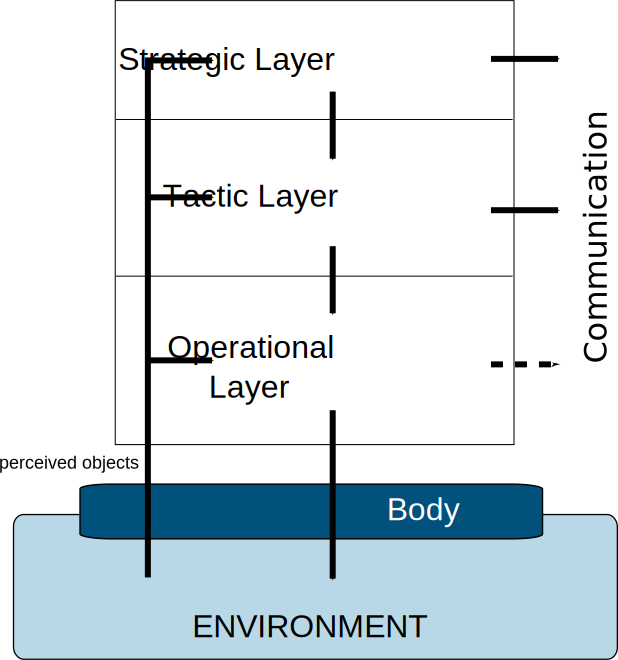
\includegraphics{standard_agent_layers}}
		\end{column}
	\end{columns}
\end{frame}

\sidecite{brooks90}
\begin{frame}[t,fragile]{{Operational Layer Example:} Subsumption Architecture}
	\begin{itemize}
	\item Priority-ordering sequence of condition-action pairs.
	\item Mostly contributes to the lower level in the three-layer architecture. 
	\end{itemize}
	\vspace{.25cm}
	\begin{columns}[t]
		\begin{column}{.39\linewidth}
			\begin{lstlisting}[basicstyle=\scriptsize]
if condition1
   action1
else if condition2
   action2
else
   ...
			\end{lstlisting}
		\end{column}
		\begin{column}{.59\linewidth}
			\raisebox{-\height}{\includegraphicswtex[width=\linewidth]{subsomption}}
		\end{column}
	\end{columns}
\end{frame}

\sidecite{Helbing.1997,Reynolds.99,buisson.abmtrans13}
\begin{frame}[t]{{Tactic Layer Example:} (Social) Force Models}
	\begin{itemize}
	\item Repulsive forces are computed and summed for obtaining the safer direction.
	\item Mostly contributes to the two lower layers of the three-layer architecture. 
	\end{itemize}
	\begin{columns}
		\begin{column}{.7\linewidth}
			\centering
			{\smaller\smaller$\vec{f} = \vec{f}_1 + \vec{f}_2 + \epsilon_1 =
				\left( \sum^k_{i=1} \dfrac{\alpha_i.\widehat{c-a_i}}{|\overrightarrow{c-a_i}|} \right)
				+ \left( \dfrac{\beta.\overrightarrow{\dfrac{\sum^k_{i=1} a_i}{k} - c}}{\left|\overrightarrow{\dfrac{\sum^k_{i=1} a_i}{k} - c}\right|^2} \right)
				+ \epsilon_1
			$}
		\end{column}
		\begin{column}{.2\linewidth}
			\centering
			{\smaller\smaller$\theta =
				\dfrac{\sum^k_{i=1} \theta_i}{k}
				+ \epsilon_2
			$}
		\end{column}
	\end{columns}
	where: $c$ is the current agent, $(a_1,\cdots,a_k)$ are the perceived agents, $\theta_i$ is the orientation of $a_i$
	\begin{center}
			\begin{tabular}{c@{\hspace{2em}}c@{\hspace{2em}}c@{\hspace{2em}}c@{\hspace{2em}}c}
				\includegraphicswtex[width=.15\linewidth]{boids_separation} &
				{\Huge $+$} &
				\includegraphicswtex[width=.15\linewidth]{boids_cohesion} &
				{\Huge $+$} &
				\includegraphicswtex[width=.15\linewidth]{boids_alignment} \\
				\small separation $\vec{f}_1$ & &
				\small cohesion $\vec{f}_2$ & &
				\small alignment $\theta$ \\
			\end{tabular}
	\end{center}
\end{frame}

\sidenote{\cite{Rao95}, Image Claude Sonnet 4.6}
\figureslide{{Stategic Layer Example:} Belief, Desire, Intention (BDI) Architecture}{bdi_rao_lifecycle}

\sidecite{Harel.87.statechart,Baum66,Rumbaugh99}
\begin{frame}[t,fragile]{{Multilayer Example:} State-Transition Diagrams}
	\begin{itemize}
	\item Define the behavior in terms of states and transitions
	\item Actions may be trigerred on transitions or states
	\item Markov models \cite{Baum66} or activity diagrams \cite{Rumbaugh99} may be used in place of state-transition diagrams
	\end{itemize}
	\begin{columns}
		\begin{column}[t]{.4\linewidth}
			\begin{sarllisting}[basicstyle=\tiny]
agent VaacumRobot {

  var state = Iddle

  on Perception
     [state == Navigating &&
      occurrence.contains(Durty)] {
    state = Cleaning
    suck()
  }

  on Perception
     [state == Cleaning &&
      occurrence.contains(DurtyBinFull)] {
    state = ReturningToDock
    moveToDock()
  }
  ...
}
			\end{sarllisting}
		\end{column}
		\begin{column}[t]{.4\linewidth}
			\raisebox{-\height}{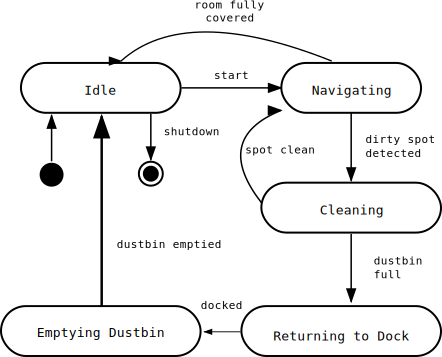
\includegraphics{vacuum_robot_state_diagram}}
		\end{column}
	\end{columns}
\end{frame}

\end{graphicspathcontext}

\endinput

